\documentclass{beamer}

\usepackage[utf8]{inputenc}
\usepackage{booktabs}
\usepackage{tabularx}
\usepackage{ragged2e}
\usepackage{xcolor}
\usetheme{Warsaw}
\usefonttheme{serif}
\institute{Bhabha Atomic Research Center}
\title{The RISC V Revolution}
\author{Sudheer K. Mohammed}
\newcolumntype{L}[1]{>{\RaggedRight\arraybackslash}p{#1}}
\newcolumntype{Y}{>{\RaggedRight\arraybackslash}X}
\begin{document}
\begin{frame}[plain]
 \maketitle
\end{frame}
\begin{frame}[plain]
\frametitle{Outline} % The title of the frame
\tableofcontents
\end{frame}
\section{Introduction}
\begin{frame}
\frametitle{Introduction}
\begin{enumerate}
\item The Duopoly (x86 vs ARM)(CISC vs RISC)
\pause
\item The patent restrictions
\pause
\item The academic restrictions (The Origins at UC Berkeley (2010))
\pause
\item open-source ISA from scratch
\end{enumerate}
\end{frame}
\subsection{Why RISC V Matters?}
\begin{frame}
\frametitle{Why RISC V Matters}
\begin{enumerate}
\item \textbf{No Licensing Fees:} Companies and researchers can design custom processor cores without paying royalties to vendor companies.

\item \textbf{Geopolitical Neutrality:} Being open-source, it reduces dependence on single corporate vendors or foreign export-control regulations.

\item \textbf{Academic \& Commercial Adoption:} It is widely used in microcontrollers, hard drive controllers (e.g., Western Digital), AI accelerators, automotive chips, and embedded systems, with growing support for Linux and Android desktop/server platforms.
\end{enumerate}

\end{frame}
\subsection{History of RISC V}
\begin{frame}
\frametitle{History of RISC V}
\begin{enumerate}
\item RISC-V was born in May 2010 at the University of California, Berkeley. Lead researchers Krste Asanović, Andrew Waterman, Yunsup Lee, and computer architecture pioneer David Patterson needed an Instruction Set Architecture (ISA) for research and teaching.
\item "V" stands for the fifth major RISC architecture designed at UC Berkeley (earlier versions included RISC-I and RISC-II in the 1980s, which helped lay the groundwork for modern processors).
\item RISC-V Foundation was established to manage and standardize the architecture collaboratively,(2015)
\item Transition to RISC-V International (2019–Present)(Switzerland) 
\item Adoption by Academia and Industry
\end{enumerate}
\end{frame}
\section{Architecture and Features}
\begin{frame}[plain]
  \frametitle{Architecture and Features}
  \begin{center}
  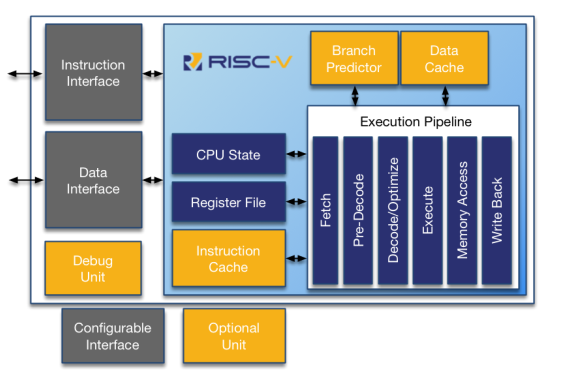
\includegraphics[width=\linewidth]{RISC-V-1}
  \end{center}
\end{frame}
\subsection{Modularity}
\begin{frame}[plain]
  \frametitle{Modularity}
\begin{enumerate}
 \item The Core Vocabulary (The Base)
 \item Extension
 \begin{itemize}
  \item The Math Helper: Add an extension for fast multiplication and division.
 \item The Decimal Helper: Add an extension for handling precise decimal numbers.
 \item The AI Accelerator: Add vector extensions to crunch massive amounts of data simultaneously for artificial intelligence.
 \end{itemize}
\end{enumerate}
\end{frame}
\section{Hardware Implementations}
\begin{frame}[plain]
\frametitle{Hardware Implementations}
\scriptsize{
    \begin{tabularx}{\textwidth}{L{2.2cm} L{2cm} L{3.2cm} L{2.2cm}}
        \toprule
        \textbf{Category} & \textbf{Key Processors \& SoCs} & \textbf{Target Applications} & \textbf{OS Support} \\
        \midrule
        \textbf{Micro controllers} & ESP32-C3/C6, WCH CH32V003, SiFive E20 & Smart home IoT, sensors, wearables, automation & Bare-metal, FreeRTOS, Zephyr \\
        \textbf{Edge AI \& Vision} & Canaan Kendryte K230, Sipeed Maix Series & Smart cameras, robotics, computer vision & Lightweight Linux, RTOS \\
        \textbf{Application CPUs} & StarFive JH7110, SpacemiT K1, SiFive P550 & Developer SBCs, laptops, workstations & Debian, Ubuntu, Fedora, Android \\
        \textbf{Cloud \& Datacenter} & Sophgo SG2042, Ventana Veyron, Tenstorrent & Hyperscale cloud, HPC, LLM inference & Enterprise Linux (Ubuntu, Fedora) \\
        \bottomrule
    \end{tabularx}}
\end{frame}
\subsection{Indian scenario}
\begin{frame}
\frametitle{Indian scenario}
 \begin{itemize}
  \item SHAKTI (2018, IIT Madras): Designed for strategic, space, and defense applications;
 \item AJIT (2018, IIT Bombay): A microprocessor for industrial and robotics applications;
 \item VIKRAM (2025, ISRO-SCL): A processor developed for space applications such as navigation, guidance, and mission operations; engineered to withstand extreme space conditions;
 \item THEJAS64 (2025, C-DAC): Designed for industrial automation.
  \item Dhruva64 (2025 C-DAC)
 \end{itemize}

\end{frame}

\section{How to get Started}
\begin{frame}
\frametitle{How to get Started}
3 Paths
\begin{enumerate}
 \item Visual Simulation (Ripes)
 \item Embedded Tinkering (ESP32 C3/Raspberry pi pico V2 or SBC Milk V Mars)
 \item HDL CPU design (verilog/System verilog)

\end{enumerate}

\end{frame}

\section{Conclusion}
\begin{frame}[plain]
\frametitle{Conclusion}
\begin{itemize}
 \item \textbf{Microcontrollers \& Storage}-Complete Takeover-"Billions of chips inside hard drives (Western Digital), smart devices (Espressif), and microcontrollers already run on RISC-V."
 \item \textbf{Edge AI \& Automotive}-In Progress-"Widely used for custom AI accelerators (Meta, Tenstorrent) and automotive controllers."
 \item \textbf{Smartphones \& PC Desktops}-Early Stages-"Google has made RISC-V a top-tier architecture for Android, but mainstream consumer devices are still a few years away from matching ARM/x86 software ecosystems."
 \item \textbf{Data Centers \& Cloud }-Emerging-"Tech giants use RISC-V for specialized cloud hardware and offload processors, though x86/ARM still dominate primary server CPUs."
\end{itemize}
\end{frame}

\end{document}
